% =============================================================
% latex/zeichenfeld-datamatrix.tex
%
% \datamatrixfeld[<144-Bit-String>]{<feld-nr>}{<klartext>}{<codewords>}
%
%   Rendert ein Werkstatt-Feld zum Selber-Zeichnen eines Datamatrix-
%   Symbols (12×12). Bestandteile:
%
%   - Kopfzeile mit Feld-Nummer und Klartext-Eingabe (leer oder gefüllt)
%   - 12×12-Modul-Raster mit L-Pattern (untere und linke Kante schwarz)
%     und Zeitsignal (obere und rechte Kante alternierend) bereits
%     vorgezeichnet. Datenbereich ist nur als Hilfsraster da.
%   - Hilfstabelle mit 12 Zeilen für die Codeword-Bytes plus
%     8 Bit-Spalten zum Eintragen.
%
%   Wenn das optionale [<144-Bit-String>] mitgegeben wird, werden
%   die Datenmodule entsprechend gefüllt; sonst bleiben sie als
%   leeres Hilfsraster sichtbar. Die Codewords (vierte Pflichtparameter)
%   werden in die Hilfstabelle eingetragen, wenn sie gegeben sind.
%
% Voraussetzungen: TikZ + xstring (in praeambel.tex geladen).
% =============================================================

\makeatletter

% --- Symbol-Raster: 12×12 Module à 6mm ---
% In Symbol-Koordinaten: Zeile 0 oben, Zeile 11 unten, Spalte 0 links,
% Spalte 11 rechts. y-Achse zeigt nach unten.
\NewDocumentCommand{\@dmSymbol}{m}{%
  \begin{tikzpicture}[x=6mm, y=-6mm, every node/.style={font=\tiny}]
    % Symbol-Aussenrahmen
    \draw[black] (0, 0) rectangle (12, 12);
    %
    % Hilfsraster für Datenbereich (Spalten 1..10, Zeilen 1..10)
    \foreach \i in {1,...,11}{
      \draw[gray!40, very thin] (\i, 0) -- (\i, 12);
      \draw[gray!40, very thin] (0, \i) -- (12, \i);
    }
    %
    % L-Pattern (immer): untere Kante (Zeile 11) und linke Kante (Spalte 0)
    \foreach \c in {0,...,11}{ \fill[black] (\c, 11) rectangle (\c+1, 12); }
    \foreach \r in {0,...,10}{ \fill[black] (0, \r) rectangle (1, \r+1); }
    %
    % Zeitsignal (immer): obere Kante (gerade Spalten schwarz), rechte
    % Kante (ungerade Zeilen schwarz)
    \foreach \c in {0, 2, 4, 6, 8, 10}{ \fill[black] (\c, 0) rectangle (\c+1, 1); }
    \foreach \r in {1, 3, 5, 7, 9}{ \fill[black] (11, \r) rectangle (12, \r+1); }
    %
    % Datenmodule aus 144-Bit-String (zeilen-major, Frame-Bits werden
    % vom Frame oben nochmal überzeichnet — irrelevant, da gleicher Wert).
    \IfStrEq{#1}{}{}{%
      \foreach \r in {1,...,10}{%
        \foreach \c in {1,...,10}{%
          \pgfmathtruncatemacro{\idx}{\r*12+\c+1}%
          \StrChar{#1}{\idx}[\bit]%
          \ifnum\bit=1
            \fill[black] (\c, \r) rectangle (\c+1, \r+1);%
          \fi
        }%
      }%
    }
  \end{tikzpicture}%
}

% --- Codeword-Hilfstabelle: 12 Zeilen × 8 Bit-Kästchen ---
% Zwei separate Helper für leer und voll, weil \IfStrEq über
% Tabellen-Zeichen mit & und \\ stolpert.
\NewDocumentCommand{\@dmTabelleLeer}{}{%
  \footnotesize
  \setlength{\tabcolsep}{4pt}
  \renewcommand{\arraystretch}{1.25}
  \begin{tabular}{c | c | c c c c c c c c}
    \toprule
    \textbf{Nr.} & \textbf{Wert} &
      \textbf{\tiny 1} & \textbf{\tiny 2} & \textbf{\tiny 3} & \textbf{\tiny 4} &
      \textbf{\tiny 5} & \textbf{\tiny 6} & \textbf{\tiny 7} & \textbf{\tiny 8} \\
        &       &
      \tiny 128 & \tiny 64 & \tiny 32 & \tiny 16 &
      \tiny 8 & \tiny 4 & \tiny 2 & \tiny 1 \\
    \midrule
    \@dmEmptyRow{1}\\\@dmEmptyRow{2}\\\@dmEmptyRow{3}\\%
    \@dmEmptyRow{4}\\\@dmEmptyRow{5}\\\@dmEmptyRow{6}\\%
    \@dmEmptyRow{7}\\\@dmEmptyRow{8}\\\@dmEmptyRow{9}\\%
    \@dmEmptyRow{10}\\\@dmEmptyRow{11}\\\@dmEmptyRow{12}\\
    \bottomrule
  \end{tabular}%
}

\NewDocumentCommand{\@dmTabelleVoll}{m}{%
  \footnotesize
  \setlength{\tabcolsep}{4pt}
  \renewcommand{\arraystretch}{1.25}
  \begin{tabular}{c | c | c c c c c c c c}
    \toprule
    \textbf{Nr.} & \textbf{Wert} &
      \textbf{\tiny 1} & \textbf{\tiny 2} & \textbf{\tiny 3} & \textbf{\tiny 4} &
      \textbf{\tiny 5} & \textbf{\tiny 6} & \textbf{\tiny 7} & \textbf{\tiny 8} \\
        &       &
      \tiny 128 & \tiny 64 & \tiny 32 & \tiny 16 &
      \tiny 8 & \tiny 4 & \tiny 2 & \tiny 1 \\
    \midrule
    #1
    \bottomrule
  \end{tabular}%
}

% Eine einzelne leere Zeile in der Codeword-Tabelle.
\NewDocumentCommand{\@dmEmptyRow}{m}{%
  #1 & \fbox{\rule{0pt}{1.6ex}\hspace{1.6em}} &
    \fbox{\rule{0pt}{1.6ex}\hspace{0.4em}} &
    \fbox{\rule{0pt}{1.6ex}\hspace{0.4em}} &
    \fbox{\rule{0pt}{1.6ex}\hspace{0.4em}} &
    \fbox{\rule{0pt}{1.6ex}\hspace{0.4em}} &
    \fbox{\rule{0pt}{1.6ex}\hspace{0.4em}} &
    \fbox{\rule{0pt}{1.6ex}\hspace{0.4em}} &
    \fbox{\rule{0pt}{1.6ex}\hspace{0.4em}} &
    \fbox{\rule{0pt}{1.6ex}\hspace{0.4em}}%
}

% --- Komplettes Werkstatt-Feld ---
% \datamatrixfeldleer{<feld-nr>}      → leeres Feld zum Selber-Zeichnen
% \datamatrixfeldvoll{<feld-nr>}{<text>}{<bits>}{<tabelle>}
%                                      → vorbefüllt
\NewDocumentCommand{\datamatrixfeldleer}{m}{%
  \par\noindent
  \begin{minipage}{\linewidth}
    \rule{\linewidth}{0.4pt}\par\smallskip
    \textbf{\large Feld #1}\hfill
    \textbf{Inhalt:}~\framebox[10em]{\strut}\par
    \medskip
    \begin{minipage}[t]{0.50\linewidth}\centering\@dmSymbol{}\end{minipage}\hfill
    \begin{minipage}[t]{0.46\linewidth}\@dmTabelleLeer\end{minipage}
  \end{minipage}\par
  \vspace{1.2em}
}

\NewDocumentCommand{\datamatrixfeldvoll}{m m m m}{%
  \par\noindent
  \begin{minipage}{\linewidth}
    \rule{\linewidth}{0.4pt}\par\smallskip
    \textbf{\large Feld #1}\hfill
    \textbf{Inhalt:}~\texttt{#2}\par
    \medskip
    \begin{minipage}[t]{0.50\linewidth}\centering\@dmSymbol{#3}\end{minipage}\hfill
    \begin{minipage}[t]{0.46\linewidth}\@dmTabelleVoll{#4}\end{minipage}
  \end{minipage}\par
  \vspace{1.2em}
}

% --- Farbig markiertes Symbol (mit Codeword-Pastellfarben + Bit-Nrn) ---
% #1 = Pfad zu einer .tex-Datei mit den TikZ-Modul-Befehlen,
%      generiert von code/tag13/gen_colored.py
% Frame (L-Pattern, Zeitsignal) wird hier komplett gezeichnet.
\NewDocumentCommand{\@dmSymbolColored}{m}{%
  \begin{tikzpicture}[x=8mm, y=-8mm, every node/.style={font=\tiny}]
    % Symbol-Aussenrahmen
    \draw[black] (0, 0) rectangle (12, 12);
    % L-Pattern (immer schwarz): untere Kante + linke Kante
    \foreach \c in {0,...,11}{ \fill[black] (\c, 11) rectangle (\c+1, 12); }
    \foreach \r in {0,...,10}{ \fill[black] (0, \r) rectangle (1, \r+1); }
    % Zeitsignal
    \foreach \c in {0, 2, 4, 6, 8, 10}{ \fill[black] (\c, 0) rectangle (\c+1, 1); }
    \foreach \r in {1, 3, 5, 7, 9}{ \fill[black] (11, \r) rectangle (12, \r+1); }
    % Hilfsraster für Datenbereich
    \foreach \i in {1,...,11}{
      \draw[gray!40, very thin] (\i, 1) -- (\i, 11);
      \draw[gray!40, very thin] (1, \i) -- (11, \i);
    }
    % Datenmodule mit Codeword-Färbung + Bit-Nummern (extern generiert)
    \input{#1}
  \end{tikzpicture}%
}

% --- Tabelle mit Codeword-Farbmarkern (kleine farbige Box pro Zeile) ---
% Aufrufer übergibt 12 Tabellenzeilen, die diese Form haben:
%   \cwrow{<Nr.>}{<Wert>}{<b1>}...{<b8>}
\NewDocumentCommand{\@dmTabelleVollFarbig}{m}{%
  \footnotesize
  \setlength{\tabcolsep}{3pt}
  \renewcommand{\arraystretch}{1.3}
  \begin{tabular}{c | c | c | c c c c c c c c}
    \toprule
    & \textbf{Nr.} & \textbf{Wert} &
      \textbf{\tiny 1} & \textbf{\tiny 2} & \textbf{\tiny 3} & \textbf{\tiny 4} &
      \textbf{\tiny 5} & \textbf{\tiny 6} & \textbf{\tiny 7} & \textbf{\tiny 8} \\
    & & &
      \tiny 128 & \tiny 64 & \tiny 32 & \tiny 16 &
      \tiny 8 & \tiny 4 & \tiny 2 & \tiny 1 \\
    \midrule
    #1
    \bottomrule
  \end{tabular}%
}

% Hilfs-Macro für eine farbige Tabellenzeile.
% #1=Farbe, #2=Nr, #3=Wert, #4=8-Zeichen-Bit-String "01001001"
\NewDocumentCommand{\cwrow}{m m m m}{%
  \tikz[baseline=-0.5ex]\fill[#1] (0,0) rectangle (0.5, 0.3); &
  #2 & #3 &
  \StrChar{#4}{1} & \StrChar{#4}{2} & \StrChar{#4}{3} & \StrChar{#4}{4} &
  \StrChar{#4}{5} & \StrChar{#4}{6} & \StrChar{#4}{7} & \StrChar{#4}{8} \\
}

\NewDocumentCommand{\datamatrixfeldfarbig}{m m m m}{%
  % #1 = Feldnummer
  % #2 = Klartext
  % #3 = Pfad zu colored-tex-Datei
  % #4 = Tabellenzeilen (mit \cwrow-Aufrufen)
  \par\noindent
  \begin{minipage}{\linewidth}
    \rule{\linewidth}{0.4pt}\par\smallskip
    \textbf{\large Feld #1}\hfill
    \textbf{Inhalt:}~\texttt{#2}\par
    \medskip
    \begin{minipage}[t]{0.55\linewidth}\centering\@dmSymbolColored{#3}\end{minipage}\hfill
    \begin{minipage}[t]{0.42\linewidth}\@dmTabelleVollFarbig{#4}\end{minipage}
  \end{minipage}\par
  \vspace{1.2em}
}

% --- Leere Tabelle mit Codeword-Farbmarkern ---
% 12 Zeilen mit Pastellmarker links + leeren Boxen rechts (Wert-Box + 8 Bit-Boxen).
% Farben müssen mit den COLORS in code/tag13/gen_colored.py übereinstimmen.
\NewDocumentCommand{\@dmEmptyRowFarbig}{m m}{%
  % #1 = Farbe, #2 = Nr.
  \tikz[baseline=-0.5ex]\fill[#1] (0,0) rectangle (0.5, 0.3); &
  #2 & \fbox{\rule{0pt}{1.6ex}\hspace{1.6em}} &
    \fbox{\rule{0pt}{1.6ex}\hspace{0.4em}} &
    \fbox{\rule{0pt}{1.6ex}\hspace{0.4em}} &
    \fbox{\rule{0pt}{1.6ex}\hspace{0.4em}} &
    \fbox{\rule{0pt}{1.6ex}\hspace{0.4em}} &
    \fbox{\rule{0pt}{1.6ex}\hspace{0.4em}} &
    \fbox{\rule{0pt}{1.6ex}\hspace{0.4em}} &
    \fbox{\rule{0pt}{1.6ex}\hspace{0.4em}} &
    \fbox{\rule{0pt}{1.6ex}\hspace{0.4em}}%
}

\NewDocumentCommand{\@dmTabelleLeerFarbig}{}{%
  \footnotesize
  \setlength{\tabcolsep}{3pt}
  \renewcommand{\arraystretch}{1.3}
  \begin{tabular}{c | c | c | c c c c c c c c}
    \toprule
    & \textbf{Nr.} & \textbf{Wert} &
      \textbf{\tiny 1} & \textbf{\tiny 2} & \textbf{\tiny 3} & \textbf{\tiny 4} &
      \textbf{\tiny 5} & \textbf{\tiny 6} & \textbf{\tiny 7} & \textbf{\tiny 8} \\
    & & &
      \tiny 128 & \tiny 64 & \tiny 32 & \tiny 16 &
      \tiny 8 & \tiny 4 & \tiny 2 & \tiny 1 \\
    \midrule
    \@dmEmptyRowFarbig{red!15}    {\phantom{0}1}\\
    \@dmEmptyRowFarbig{orange!20} {\phantom{0}2}\\
    \@dmEmptyRowFarbig{yellow!30} {\phantom{0}3}\\
    \@dmEmptyRowFarbig{lime!20}   {\phantom{0}4}\\
    \@dmEmptyRowFarbig{green!20}  {\phantom{0}5}\\
    \@dmEmptyRowFarbig{teal!20}   {\phantom{0}6}\\
    \@dmEmptyRowFarbig{cyan!20}   {\phantom{0}7}\\
    \@dmEmptyRowFarbig{blue!15}   {\phantom{0}8}\\
    \@dmEmptyRowFarbig{violet!15} {\phantom{0}9}\\
    \@dmEmptyRowFarbig{magenta!15}{10}\\
    \@dmEmptyRowFarbig{pink!25}   {11}\\
    \@dmEmptyRowFarbig{brown!20}  {12}\\
    \bottomrule
  \end{tabular}%
}

% --- Werkstatt-Feld in farbig + leer ---
% Pastell-Symbol mit "c/b"-Labels (kein schwarzes Bit gesetzt) plus
% leere farbige Hilfstabelle. Greta trägt selbst Wert + Bits ein und
% schwärzt die Module passend zu ihrem Codeword.
\NewDocumentCommand{\datamatrixfeldfarbigleer}{m m}{%
  % #1 = Feldnummer
  % #2 = Pfad zu colored-tex-Datei (typisch blank_colored.tex)
  \par\noindent
  \begin{minipage}{\linewidth}
    \rule{\linewidth}{0.4pt}\par\smallskip
    \textbf{\large Feld #1}\hfill
    \textbf{Inhalt:}~\framebox[10em]{\strut}\par
    \medskip
    \begin{minipage}[t]{0.55\linewidth}\centering\@dmSymbolColored{#2}\end{minipage}\hfill
    \begin{minipage}[t]{0.42\linewidth}\@dmTabelleLeerFarbig\end{minipage}
  \end{minipage}\par
  \vspace{1.2em}
}

% --- Cheat-Sheet für Datamatrix: Anatomie + Utah-Form ---
\NewDocumentCommand{\datamatrixcheatsheet}{}{%
  \par\smallskip
  \noindent\textbf{\small Spickzettel — Datamatrix-Anatomie}\par
  \smallskip
  \noindent
  \begin{minipage}[t]{0.50\linewidth}
    \footnotesize
    \textbf{12$\times$12-Symbol:} 5 Datenbytes + 7 Prüfbytes (ECC).
    L-Pattern unten und links (immer schwarz), Zeitsignal oben und
    rechts (alternierend). Datenbereich ist die $10\times 10$-Innen\-
    fläche.
    \par\smallskip
    \textbf{Utah-Form:} jedes 8-Bit-Codeword wird als L-förmiger
    Block gesetzt (3$\times$3-Quadrat ohne oben-rechts):
    \begin{center}
    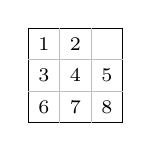
\begin{tikzpicture}[x=4mm, y=-4mm, font=\scriptsize]
      \draw (0,0) rectangle (3,3);
      \foreach \i in {1,2}{ \draw[gray!50] (\i,0) -- (\i,3); \draw[gray!50] (0,\i) -- (3,\i); }
      \node at (0.5,0.5) {1}; \node at (1.5,0.5) {2};
      \node at (0.5,1.5) {3}; \node at (1.5,1.5) {4}; \node at (2.5,1.5) {5};
      \node at (0.5,2.5) {6}; \node at (1.5,2.5) {7}; \node at (2.5,2.5) {8};
    \end{tikzpicture}
    \end{center}
    Bit 1 = MSB (128), Bit 8 = LSB (1).
  \end{minipage}\hfill
  \begin{minipage}[t]{0.47\linewidth}
    \footnotesize
    \textbf{Stellenwert-Tabelle:}
    \par\smallskip
    \begin{tabular}{c | c c c c c c c c}
      \textbf{Bit} & 1 & 2 & 3 & 4 & 5 & 6 & 7 & 8 \\
      \textbf{Wert} & 128 & 64 & 32 & 16 & 8 & 4 & 2 & 1 \\
    \end{tabular}
    \par\smallskip
    \textbf{Beispiel:} $73 = 64 + 8 + 1$, also Bits
    \texttt{01001001}.
    \par\smallskip
    \textbf{Algorithmus:} Cursor startet bei (Zeile 4, Spalte 0).
    Sweeps abwechselnd hoch-rechts und runter-links durch das Symbol;
    pro Position eine Utah-Form. An den Symbol-Ecken vier Sonder-
    Patterns (Corner 1--4).
  \end{minipage}%
  \par\medskip
}

\makeatother
